\chapter{迷路羊群}

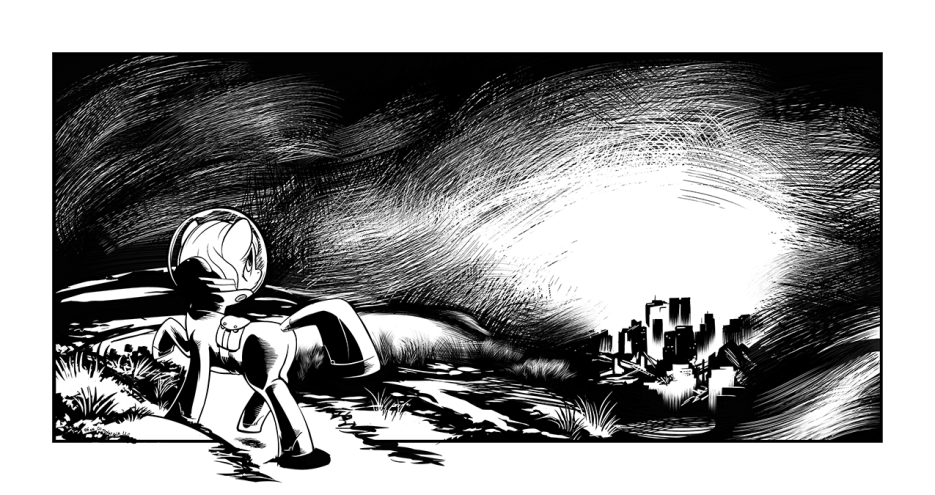
\includegraphics[width=\linewidth]{image03.png}

\begin{intro}
很久很久以前,在逐渐消亡的小马国土地上
\end{intro}

「{\rt 女士们,先生们,晚上好!这里是孤狼\footnote{孤狼 (Lonesome Pony):后面缩写为 L.P.}的52电台!虽然,野马 DJ PON-3 尥蹶子踹好了吠城 (Fillydephia) 的广播晶片,所以十马塔 (Tenpony Tower) 的广播在整个废土都收得到!但是只有在这里才有你想要听到的所有52国道新闻!}」

然后一阵悠扬的音乐持续了几秒钟。

「{\rt 以上就是大狗\footnote{大狗:这里指孤狼}能提供的全部服务了,现在回到本地新闻。嘿,小马们,你们害怕幽灵吗?也许你们应该害怕。你们记得嘉年华的故事吗?如果没听过不要紧,老朋友L.P.现在就给那些没预习功课的小马们补补课!}」

「{\rt 在52号国道最最最最最北边的地方,有一处大家不知道的农舍,赤兔们叫它嘉年华。那是一个年代久远的遗迹,但是不像它的兄弟姐妹一样,嘉年华从未真正安眠。自从我祖母记事以来,每隔一年就会有一个幽灵从那里出现,游荡在附近的山丘,邀请大家参加她的聚会。当第二天早上来临的时候,就会有小幼驹神秘地消失,然后再也回不来了。感谢那些无处不在的激光炮台,靠近嘉年华几乎是自杀。不过如果你靠得够近,就能听到在那被诅咒的谷仓里面传出音乐声,就像是整天整夜地在狂欢一般。}」

「{\rt 我的小马们,看起来似乎是有谁大喊着『我不怕幽灵!』然后冲进那派对中把整幢农舍的房顶掀翻了。非常勇敢。现在赤兔的小幼驹终于可以安心睡觉了。我很好奇这个神秘的英雄是谁,但是大家都说她也是一个幽灵。是一只在粉云之中穿着黄色防辐射服死而复生的小幼驹。干得好,黄色幽灵。你给废土解决了一个大麻烦,你面前还有一百九十九个要解决!哦,我有提到今年嘉年华的被害者安全回家了吗?塞拉斯蒂娅公主祝福我们!现在还是继续我们的小马萨克斯吧!}」

\begin{song}
我在千里之外看到指路之星,

I can see that lone star from a thousand miles away,

\medskip

它在远处向我招手叫我回家。

Calling me back home, though I've ventured far away.

\medskip

指路之星如灯塔般给我带路,

When I see that beacon shining for me all along,

\medskip

让我回到小马国回到我的家!

It calls me to Equestria and a home!
\end{song}

\horizonline

\daytimeplace{4}{00:30 AM}{盐块平原,52号国道北口}{Salt Cube Flats, Big 52 N Branch}

帕比顺着52国道一路向南,远处大城市的剪影从地平线上跃升成为一个高楼林立的巨大水泥丛林。幼驹走了整整一天,而现在阳光消逝在黑暗之中。小雌驹眼睛中闪烁着的亮粉色光芒照亮了她的道路,虽然没有阳光,但还是可以清楚地看到盐块城那个微微发光的圆顶建筑,还有几座巍峨的摩天大厦耸立在一片漆黑的废墟之中。

差不多午夜的时候,小雌驹看到一个小车队从他的方向一起往南走,大概有半打小马和非常非常奇怪的……有两个脑袋的牛跟着他们?帕比惊奇地坐在地上,等待着他们靠近。显然车队卫兵也很快发现了幼驹,毕竟她是个坐在路当中的光源。当然,卫兵做好了战斗准备。

一个穿着轻型战斗鞍具的大块头低声问着旁边的小马。「你觉得……这个就是新闻中说的那个『幽灵』吗?」

卫兵的领头,一只带着大号左轮枪的陆马耸了耸肩,举起蹄子示意车队停下来。

「不清楚,但是我不冒险,所以我们慢慢来,你们俩去旁边,另外俩站在这里,我去交涉,好好掩护我,要不然你们别想领薪水。」

两个卫兵离开车队向旁边的小路前进,绕到帕比的侧翼,同时领头走出车队,两个卫兵保持距离守在后面。小雌驹的样子看起来很诡异,一个发出粉色光芒的大圆头盔安在一个小小的黄色轮廓上,不过的确是个很明显的靶子,卫兵领队一边小心靠近,一边祈祷她的卫兵在发生什么突发状况的时候能够救她一命。

「嗨!我是快乐帕比!」幼驹举起一只蹄子向领队挥舞着。好吧,至少她看起来还算友善。

不过在废土生存指南上,不止一次强调过「有备无患——看起来友善不等于安全。」

「好吧,站在那里别动,说个不让我把你变成一堆化肥的理由。」

帕比咯咯笑着,奇怪的话总能逗乐她。「喂喂,漂漂小马爱说笑!我不叫华菲!我是帕比,你叫什么名字?」

卫兵头头迟疑着,这个幼驹只是在冒傻气还是给她设了一个精心布置的圈套?但是经验告诉她有哪里不对劲。「对,我是固体虫。你独自旅行?」不等回答,她的卫兵已经开始检查附近了。

「当然不是,我和声音先生一起!他有时候超级聪明有时候超级笨蛋,取决于……不管怎么说他知道我妈妈在哪里啦!」

「那么……这个声音先生又在哪儿?」

「在这个太空服里!看到这些灯和漂亮点点了么?他能让这些东西出现!」

固体虫仔细看了看衣服的头盔,不去管帕比那俩闪闪发光的大眼睛,的确有一个HUD,和一些高级战斗鞍具用的瞄准设备差不多。一看到这个看起来价值连城的上古装备,她很想知道一个幼驹怎么能找到这种好货?但是那粉光总让她觉得不太自在。简单地说,固体虫干了很久护卫,见过废土上的不少东西。

「这么说,你应该是从中心城来的?」

「对哦!我家的房子就在……呃……正好在山脚下的四叶镇,不过有一天它塌了,所以现在我在找我妈妈。她不在声音先生说的一个旧农场,不过他说这个大城市还有另一个大地方。所以我要去那里看看!」帕比用蹄子指着南边说。

固体虫听的时候点了几次头,举起蹄子示意车队可以安全通过。在车队开始前进的时候她说。

「你可真能聊,不是么?孤狼刚讲到你在嘉年华的大冒险\footnote{大冒险:冒险 (exploit) 和后面的爆炸 (explode) 似音}。」

「我的啥?你说那个旧农场,我没炸了那里,农场自己爆炸了,小傻瓜。」帕比咯咯笑着。「那个机器萍琪绝对是个坏蛋!虽然开始很可怕,但我可是很勇敢的哦!」

固体虫挠了挠头,不想让帕比在闲扯下去了。「呃,没错,你很棒,我很想继续聊一会儿,但是我们还有事,如果你想去盐块城,那里的尸鬼集会在圆顶里面,我想他们把那里称作『炫彩』。别在城里闲逛,城里的人不喜欢你们。不管怎么说,祝你好运,小幽灵。」

当车队路过的时候,其他小马都好奇地看着帕比,但是固体虫和一个紫色红棕的独角兽说了两句,于是他们继续前进,黄色的幼驹很吃惊地看着那些双头牛,并且拼命地挥着蹄子,一直到他们消失在夜色中,然后她继续独行向南走。

\horizonline

\daytimeplace{4}{11:30 PM}{闹市区,盐块城}{Downtown, Salt Cube City}

这里的大门只是个用沙袋和破金属片堆成的壁垒。在一个木制平台上,有只穿着金属马铠的小马坐在一挺加特林机枪后面,另外两个门卫正在检查每一个想要进盐块城的小马。最后一个穿着军官制服的独角兽则坐在一个金属小房子里面写着什么。

虽然说现在快到正午了,但是城北门外和废土其它地方一样空无一马。这次帕比早有准备,她把那个有着白苹果的铁片给卫兵看。其中一个小马走过来,另外的几个卫兵则举起了武器。

「我看看。没错,就是这个通行证。那么,你叫什么名字,来做啥?」

「我叫快乐帕比!神秘的漂漂马你叫什么呢?」

卫兵抬起头盔的面罩,一脸不爽地看着帕比。「远见下士,好了,现在可以告诉我你来干啥了吧?」

「哦,这个问题我知道!我在找我妈妈!她大概在这个方向!」帕比伸出蹄子指向那堆残破不堪的建筑给卫兵看。

「好吧,够了,还有个问题,为啥你穿着全套环境防护服?」

「哦,这个么?我困在里面出不来了,不过没关系,因为有个狠好心帮助我的神秘声音也住在里面。」然后幼驹小声对远见咬耳朵。「不过他一点也不擅长找谁,不过别和他说,因为他脾气不好。」

卫兵放下面罩耸了耸肩。「只要你不打算在闹市区引爆超聚魔法,你想怎么穿就怎么穿。欢迎来到盐块城,小鬼头。」

幼驹连忙头也不回地跑过路障,但是远见在她身后喊着。「哦,对了,提醒你一下,别接近那个圆顶,因为那里面有野生尸鬼,而且有很多辐射污染。」

「好的好滴好吧!拜拜卫兵远见先生!」帕比跟着粉色箭头的方向,从那几个摩天大楼里穿了过去。

这里的闹市区和52号国道的其它街区差不多,有卫兵在往来巡逻,防止小马们在街上火拼。还有各个不同的贸易公司在街上竖起来的广告牌。比如『水农』或者『飞驰子弹』甚至还有一些雇佣兵和附近一些部落的交易代表。这个完全开放的市场看起来就是城市的中心,不过这个城市的真正中心是那四栋经过百年战争和风雨洗礼依然屹立不倒的摩天大楼。

盐块城在战争中曾经就被一个超聚魔法击中,不过运载超聚魔法的魔法导弹似乎出了一些问题,弹头击中了城市郊区的盐块圆顶,击穿了那个圆顶建筑的房顶,然后在里面爆炸了,坚固的圆顶保护城市免受冲击波的伤害,但是城市还是受到了放射性尘埃的影响。在之后的岁月中,城市里的大多数高楼大厦都在岁月的侵蚀下一个接一个地倒塌。但是那四座基本没有受损的摩天大楼依然在城市中心屹立不倒。

这四座高塔就是盐块城权力的象征:其中两座双子楼曾经是某个大型国际贸易公司的总部,而另一个和他们差不多高的大楼是一个强大的雇佣兵公司——聘蹄 (Hired Hooves) 的总部,最后一个,也是最小的一个,上面贴着白色苹果标志的大厦。住在里面的是这个城镇的所有者。整个城镇的所有交易都要向他们交税。白苹果同时也是聘蹄的主要兵员提供者,因为聘蹄的很多士兵都是这个家族的小马。

帕比站在一个染着红色印记的帐篷面前——这个印记表示帐篷的所有者是赤兔部落。这个商店的架子里面摆满了各式各样的铠甲和肉搏兵器,一个带着旧牛仔帽的雌驹坐在帐篷中间的一个弹药箱上。

「嘿,穿得不错的小家伙,你是不是从北边来的?」雌驹很富有魅力地笑了笑,用一只蹄子推起牛仔帽。牛仔帽下面露出了她前额上的独角。而在她臀部上的可爱标记看起来像一个棒球棒。

「嗨!我叫快乐帕比!」幼驹挥着蹄子走向雌驹。她指着帐篷外面的方向说:「我从那边来!」

「我叫强攻,我想你就是孤狼昨晚提到的那个家伙。」

「呃,你说那个在音乐频道唠唠叨叨的家伙?」帕比若有所思地挠着她的头盔,「上次我就听他说什么喝纯净水很重要。」

「不,不,我是说你是新闻里面说的那个『黄色幽灵』吧?或许附近不只有一个小马穿着防辐射服闲逛?不管怎么说,你想买点啥?」

帕比皱着眉头,「为啥大家都叫我幽灵?」

强攻笑出声来:「就是你嘛,我就知道!」独角兽轻抚着自己的下巴想了一会,「不管怎么说,作为一个拆了那诅咒农场的英雄,你是不是有点年轻?实际上你这个年龄就你自己在废土上冒险可不应该……你难道是个童子军\footnote{童子军 (Crusader):可爱标记童子军的大名在废土上可谓如雷贯耳}?」

「当然不是,我是在找我妈妈!而且我不孤单呢,声音先生陪着我!」

「你妈妈?或许我可以帮你,毕竟我在闹市区认识很多小马,你妈妈叫什么名字?她可爱标记是什么?」

快乐帕比大概描述了一下。「哦,她名字叫阴雨·黛丝,她毛皮是紫色鬃毛是橙色,她的可爱标记是有着雨点的云彩!你见过她么?声音先生说她在这附近!在那边!」帕比指着那个半毁的圆顶说。

强攻摇了摇头。「抱歉,小鬼,完全不记得有这么一个可爱标记的小马,也不记得听过这个名字。」卖货的独角兽皱着眉头看着幼驹指着的方向,「你说那边?那可不是什么好地方,那里辐射很强,而且那里唯一一个比较完好的建筑物就是圆顶,听我的,你绝对不会想到圆顶附近的。」

「圆顶?那是啥?」

「那里到处都是野生尸鬼和其它可怕的东西,虽然说你穿着防辐射服不怕那里的辐射,不过最主要的问题还是那里的居民——一小撮鬼迷心窍的尸鬼。他们基本上就是个会行走的定时炸弹。虽然他们看起来暂时很文明,不过不知道什么时候他们就会发疯攻击小马。而且现在白苹果也正在想办法除掉这些快腐烂的脑袋——他们会打爆每个走出废墟的尸鬼头。但是他们没办法进去检查,如果你不免疫辐射的话,那里面就是个巨大的死亡陷阱,所以他们也束蹄无策。」

帕比皱着眉头问:「尸鬼是什么啊?」

「你……在开玩笑吗?你都不知道尸鬼是什么?」强攻看着帕比脸上的表情,然后说:「好吧,看起来你没开玩笑。尸鬼就是小马被辐射长时间影响的结果。当超聚魔法爆炸的时候,有些小马没有死掉,而是变成了某种……怎么说呢?活跳尸?或许可以说是僵尸?不管怎么说,他们其中一部分变成了野生尸鬼——这些家伙见谁吃谁。还有一些能够保持自己心智的家伙变得永生不死,但是他们身上的肉还是会腐烂,鬃毛也基本掉光。每个尸鬼看起来都像一具正在腐烂的尸体,但是却还活蹦乱跳的。而且最大的问题就是,那些神智清醒的家伙迟早也有一天,脑子里面的神经『嘎嘣』一下,然后就变成了野生尸鬼。」

帕比眉头紧皱,独角兽感觉到她似乎很害怕。

「强攻小姐……呃……如果我妈妈真的在声音先生说的那个地方,她会安全么?」

「我想……」独角兽低下了头,把眼睛藏在帽子下面不去看幼驹那双纯洁的双眸。「我不知道,小幽灵,圆顶是个危险的地方,我只是希望你听我说完之后打消去那里的念头。」

帕比昂首挺胸四蹄站直,眼中的信念无比坚定。「我必须去那里!妈妈也许就在那里,她可能有危险!」

强攻看起来没办法说服她不要去做这个自杀任务。「你和我非亲非故,我没办法叫你不要去那里,但是还是请听听我的意见。到那座高塔那里去,就是有白苹果标记的那座高塔,然后和那里的小马说你想去圆顶里面执行侦察任务,他们或许会给你一些装备和援助,让你安全一点。」

帕比微笑着回答:「好的!我知道了!等着我妈妈,我这就去救你!」幼驹飞奔出帐篷冲向白苹果塔。

\horizonline

\daytimeplace{4}{2:00 PM}{盐块圆顶,盐块城}{Salt Cube Dome, Salt Cube City}

「{\mt 警告,侦测到少量辐射,威胁等级:可忽略。}」

圆顶曾经是一个巨大的椭圆形建筑物,曾经作为一个可以同时举行数个展览会的巨型会馆。一个巨大的球形屋顶把整个建筑物包裹起来,但是现在它基本被摧毁了,剩下一些残垣断壁像是一个超大号的露天体育馆。

在圆顶的正面有一条小道,小道上有一堆石头拱门的残骸。这些残骸看起来曾经是抛光的大理石柱,但是现在只剩下一堆碎石。帕比站在小道的面前,看着罗盘上的粉色箭头。

「好吧声音先生,我们现在要做什么来着?」

「{\mt 士气部分部已经到达,主要任务目标完成。}」

「我知道我们到这里了,我说接下来我们该做什么?」

「{\mt 次要任务目标:和尸鬼交涉并且/或者解决他们。警告,侦测到少量辐射,威胁等级:可忽略。}」

「那么,我们找到那些尸鬼,然后问他们妈妈在哪里,然后赶他们走开?」

「{\mt 肯定。这个说法很接近了。}」

「赞!我喜欢有计划的感觉,我们开工吧!」帕比走进大厅然后大喊,「嘿!尸鬼小马!」她声音的回音在巨大建筑里面回响,但是看起来却没有回答,于是穿黄衣的幼驹慢慢走到大厅的台阶下面。

「{\mt 警告,侦测到大量辐射,威胁等级:可忽略。}」

「嘿,我觉得我看到有谁在那些雕像后面走!喂,你等等!」帕比冲向那个黑影躲藏的大理石柱子后面,她看到一个黑影于是大叫道:「嗨,我是快乐帕比,你有看到我妈……」

是他!是那个家伙!马尾伯爵!他就站在她面前,虽然比她记忆中的还要更丑更可怕。

「{\mt 警告,侦测到敌对生物,野生尸鬼,距离 \SI{2}{m},威胁等级:低。}」

那个生物回头看着帕比的脸,黄色的口水从他嘴里面流出来,他看起来很疑惑,不知道下一步该干啥。

帕比满脸惊恐地看着那个生物后退一步。

「为……为什么你还跟着我?走开!走开!!」

那生物面对帕比嘶吼着低下头,而后者则撒开四蹄以她最快的速度逃命。

不过她跑得还是不够快。

头盔的设计就是为了抵御外来伤害,所以这个野兽的攻击只是让帕比幼小的心灵受到了惊吓。一口腐烂的,锯齿状的牙齿刮擦着她头盔上的画面,以及那尖锐的摩擦声就足够把她吓傻。

「咿咿咿咿咿咿呀呀呀呀呀呀……!」帕比本能地用力踢着那个尸鬼,但是那东西比一个幼驹实在重太多。

「石头,给我石头!快!」

幼驹一边尖叫着一边用双蹄抓起漂浮到她面前的「命运之石」,然后用力地砸向那个怪物。

「给我停下,停下!快停下!」

几分钟之后,帕比还在用石头用力砸着一滩棕色肉泥,这东西曾经是一个小马的脑袋。头盔上的划痕和一些划破的衣服在自动修复法术的作用下已经消失。最后尸鬼已经完全不会动,而帕比也需要喘口气。

虽然刚刚好可怕,但是马尾伯爵已经被消灭了!她最糟糕的梦魇已经消失,再也不用逃跑或者躲躲藏藏了!帕比大大松了一口气,然后把自己的视线从死掉的尸鬼身上挪开。

不过她马上就注意到另外三个尸鬼正在用同样空洞的眼神流着口水看着她。

「{\mt 警告,侦测到敌对生物,数量 3,最近目标:\SI{12}{m}。}」

「喂,声音先生。你说的无解还是误劫的那东西是啥意思?」

「{\mt 误解,错误的理解一个词语和句子的意思。}」

帕比一边看着三个尸鬼一边慢慢点点头。

「那好,你说的马尾伯爵到底是什么意思?」

「{\mt 敌对生物数量。在感应器范围内有攻击性的生物。现在敌对生物数量3,种类:野生尸鬼,威胁等级:中等。}」

帕比叹了一口气,举起石头冲向尸鬼,而尸鬼也同样冲了过来。

\horizonline

\daytimeplace{4}{2:30 PM}{盐块圆顶,盐块城}{Salt Cube Dome, Salt Cube City}

「{\mt 警告,外衣密封性遭到破坏。警告,侦测到幼角药剂。警告,罗盘无法工作。警告,物品管理系统离线。警告,能量水晶遭到破坏。能量火花剩余29.06\%。警告,侦测到致死剂量辐射,威胁等级:可忽略。主体已死亡,生体指数稳定。检测完毕。}」

帕比完全站在一个大屠杀场景的中央,身上沾满了粘液和碎肉,三个尸鬼的无头尸体横七竖八地躺在她身边。这场战斗打了这么久的原因是因为帕比站在了强辐射区中间,只是尸鬼的重生能力最后还是输给了粉色药剂和帕比防辐射服的自动修复魔法。而且比起那些只知道乱咬的尸鬼,帕比能够用石头不停地打他们的脑袋。不过她也和一个沙袋一样被踢咬了很多下。她的臀部大半都被吃掉了,剩下大团粉雾包裹着那里。

「我说,声音先生……你确定妈妈在这里?」

「{\mt 肯定,准确位置:斗志部建筑编号:00201——盐块城圆顶。}」

「好吧……好滴……好得……」帕比已经听够了『肯定』,在战斗中精疲力竭的她现在很不爽地踢着地上的土。「为啥我现在只想哭呢?」

几个小马身影出现在大厅的另一端,他们看起来似乎在低声耳语着,其中之一拿着一杆猎枪,而另一个小心地接近黄色幼驹,帕比伸出蹄子抓住落在一边的「命运之石」,但是她现在很累,只想再多躺一会。「拜托……别欺负人家……走开……我是乖孩子……」

帕比看清了走进的那个小马,它是另一个尸鬼,但是却和其他尸鬼不太一样,这一个穿着和给她外套的雌驹一样的白大褂,就是脏了很多。而且在它的眼中可以看到智慧的光芒,而且最后一点,它说话了。

「嘿,你还好吗小家伙?这里非常危险。」这个小马的声音就像是粉笔在黑板上的刮擦声音,不过帕比依稀觉得它应该是雌驹。

「我说,软气!趁她还没受辐射伤之前赶紧把这个小家伙从辐射区拖出来!我们还有辐特宁之类的么?」

「我觉得没有必要,躲开那些粉云,那东西看起来很熟悉,我可以肯定那是什么危险品。」

跑来侦查的小马听到之后停了下来,歪着头看着那团粉雾。

「我的天,我的眼睛坏了么?」尸鬼说着绕了一圈,那些粉雾很快就消失了,就好像幼驹的外套在自我修复过程中把粉雾吸了回去一样。

「{\mt 外衣密封性恢复。警告,侦测到致死剂量辐射,威胁等级:可忽略。}」

看着尸鬼雌驹慢慢靠近,帕比依然举着她的小小『武器』。幼驹想还是应该先礼后兵。「我……那个……我想这些丑丑马不是你的朋友吧?」

「你是想说『尸鬼』吧,小家伙。好吧,确切的说他们曾经是我的朋友,不过我觉得你现在是帮了他们一个忙。所以,没有好马受伤。」

尸鬼雌驹站在帕比面前看着头盔里面,幼驹虽然看起来有些不开心,但是完全没有任何伤痕或者腐烂的迹象。只是在她的眼眸之中燃烧着明亮的粉色,而且她的说话声音也比普通孩子大那么一点。「你还真是个奇怪的尸鬼,我叫桃花,你叫什么名字?」

「呃,哦哦,对哦,我叫快乐帕比,我正在找我妈妈,她应该在这附近,但是我见到的都是些丑马。」

桃花挥着蹄子招呼她的伙伴:「软气,别发呆赶紧过来!」

然后她回头继续和黄色的幼驹说。「你能不说我们是丑丑马么,叫我们尸鬼,而且如果你妈妈在这里她也应该是个尸鬼,或者是个超级史莱姆什么的。你妈妈叫什么名字?」

「这个问题我知道!她叫阴雨·黛丝而且超级酷!你见过她么?」

走过来的那个家伙听到之后说:「阴雨……阴雨……这个名字听起来好熟,你让我好好想想,我好像记得有这个名字?」

帕比一脸惊奇地看着软气,「真的?拜托拜托拜托!她在哪?」

「喂喂,等一下,我说了我记得不太清楚!我记性已经不如从前那么好了……不管怎么说,如果你不想再碰上其他野生尸鬼,那么我们还是赶快走吧,去炫彩大厅 (The Glow)。」

桃花点了点头:「没错,我们赶紧走吧,反正我们找到要找的东西了,呃,帕比,你从哪儿来的?」

「中心城!」帕比自豪地挺起胸。中心城是最棒的城市,为什么不自豪呢?

两个尸鬼都皱起了眉头,桃花扭开了脸,而软气长叹一声。

「哦,原来你是那种东西啊。」桃花喃喃自语着。「烂透了的战争。」

\horizonline

\daytimeplace{4}{3:00 PM}{炫彩大厅,盐块城}{The Glow, Salt Cube City}

炫彩大厅其实只是这个圆顶中心的一个尖顶小屋。这里的圆顶早已不复存在,满地都是各种废墟。小屋上有着三个粉色的蝴蝶标记,小屋的坚固材料在两个世纪的风吹雨打中都没有损坏。

不过这里叫做炫彩大厅的原因不是因为小屋也不是因为尸鬼,这里正中央有一个十二米高的大方块正发出绿色的荧光\footnote{辐射荧光:切伦科夫效应,但不是所有辐射现象都会有明显的切伦科夫效应,所以该解释仅供参考}。

「{\mt 警告,辐射等级超出量程,探测器紧急关闭以避免受到永久损坏。威胁等级:可忽忽忽忽忽……}」

头盔的HUD忽然消失了,帕比皱起了眉头。然后又耸耸肩,就算是声音先生也许有时候也想要去睡一觉吧。

中间的方块此刻吸引了帕比的全部注意力。那个透明的方块发出超级漂亮的光芒,幼驹希望能有个一样的小方块放在自己卧室里面,这东西一定能吓跑她床底下那些坏怪物。然后有那么一瞬间幼驹想起自己的房子,只觉得鼻子一酸。但是想到自己是一个正在执行任务的小马,她没有时间去哭鼻子,所以她问道:「那个漂亮的发光方块是什么?我也能有个发光方块么?拜托,超级拜托?」

软气笑出声来:「我想不行,帕比,不过如果你做个乖孩子我可以给你点儿别的,可以么?」

帕比开心的蹦来蹦去:「礼物?给我的?快给我,给我,给我!」

「好,好……不过做个乖孩子,好么?首先我们要和沙盒聊聊,然后我们去找找看阴雨小姐。」

帕比立刻安静下来,乖乖地跟在软气和桃花身边。「那个……就算你们超级丑,但是你们超级有趣而且超级和善!」

桃花一脸的不爽:「好吧,多谢夸奖,怪物小姐,好了,就是他了,沙盒,这个营地的头头。」

另一个尸鬼正在看着一摞纸,并且不断地挠着头。

「就算有时候他看起来有点秀逗,不过他也比其他科学家要聪明很多。嘿,老大,我们有客人了。」

尸鬼的领导穿着一件老旧的白大褂,戴着一副眼镜。他看起来对那些纸上的内容显得有些不安。他看都没看帕比一眼就回答道:「真好,告诉他我们的规矩,警告他别去闹市区,很抱歉我现在不想聊天。」

帕比咯咯笑着走到他面前,看着他的脸说:「呀,丑丑马也会说奇怪的话!嗨,我叫快乐帕比,你叫我帕比也行!你见到我妈妈了么?」

桃花一回头那幼驹就跑过去了,想要拦都拦不住。尸鬼卫兵正想解释的时候,却被她头领阻止了。沙盒推了推他的眼镜,盯着帕比研究了一会之后,忽然大叫起来。

「哦,我的露娜小蹄子!这难道是又一套能正常工作的Mark
VI么?这可真是个奇迹,不是么?」

桃花和软气都一脸茫然的看着他们的老大,但是沙盒完全不在意其他小马的表情,只是继续说下去:「这东西本来设计目的是为了保护幼驹不受到辐射尘的影响,里面安装了最先进的医疗魔法护符和最新的逻辑魔法回路——你知道的,避难厩科技 (Stable Tech) 制造的哔哔小马\footnote{哔哔小马 (PipBuck):详细介绍可以参考 \emph{FoE} 序章的内容}用的那种。」尸鬼摇了摇头,他的兴奋之情变成了哀伤,「但是我们没有预料到的是,这些科技和魔法在粉色药剂下产生的结果:这件外套的医疗补给和医疗魔法护符缓和了毒气的致命效果,创造了最佳的……恩……『融合』环境。」

那个科学家转头对其他两个尸鬼说:「你们听说过幽灵羊群么?」两个小马摇摇头,沙盒把蹄子放在帕比肩膀上,让她站在他身边。

「那是女神陨落大概一个月之后的事情,一小群和这个孩子一样穿着黄色防护服的幼驹离开中心城,他们之中大多数都已经因为突变而失去心智,而其他的幼驹完全不知道发生了什么。他们的确是幽灵:因为中心城的大屠杀而失去自己双亲,他们在一起只是因为他们认识的其他小马都已经死了。就这样漫无目标的一路向南前进,虽然路上遇到一些幸存者,但是那些已经发疯的小孩只知道把他们见到的所有活物撕成碎片。其他的孩子……他们只是不想被单独留下而跟着马群走。」

桃花吓得后退一步。「但是她看起来没那么危险啊。」

沙盒冷笑一声,继续讲他的故事:「他们和我们尸鬼一样基本是不死的,不同的是,他们和中心城尸鬼一样,只要他们不被扯的四分五裂,就能够完全重生。而且更糟糕的是,MK VI 有非常先进的自我修复魔法可以让他们自行再生受损肢体。他们简直是黄色的小魔鬼。」

软气摸着下巴问:「但是如果他们这么无敌,他们现在又在哪里?」

「我不太清楚,他们大多数还是被射杀了。至少,如果能够在砍掉他们脑袋的同时击毁他们的主魔法回路和备份系统就可以搞定。虽然说起来简单,但是如果你不清楚这东西构造的话完全做不到。不过不管怎么说,他们在肆虐几个星期之后,还是离开了,我们应该好好悼念他们,这些被这个该诅咒的战争遗留在这个死亡大陆上的可怜小家伙。」

沙盒轻轻拍着帕比的头盔,幼驹虽然听懂一部分,但是却没完全听懂。「我不喜欢这个故事,这个故事让我觉得很伤心。」

沙盒只是叹了口气,轻轻拥抱着帕比。

「别担心,小家伙,只是个枕边故事,别让老马的鬼故事把你吓坏了,我想我找到了那个萍琪玩偶了,好吧,我们玩个游戏,你告诉我为什么来这里,我给你那个玩偶,好么?」

帕比的脸上露出一个大大的笑容,那个幽灵故事早已经被小幼驹忘在脑后。「当然!我来找我妈妈,她名字叫阴雨·黛丝,她是最棒的小马!」

帕比又想了想,然后补充道:「哦哦,还有,我来这里告诉尸鬼们离开这里别回来了!你们有见过尸鬼么?丑丑马老大?」

桃花以蹄覆面。

~\vfill

\begin{note}
    升级 (Lv 2)

    新增加专长:小小战士——你在投掷,近战和肉搏上得到 5\% 奖励加成。
\end{note}



